\section{Results and Discussion}
\label{sec:results}

The results are presented in the same order as the scientific question. First, the sealed matched TEST comparison establishes whether K1 retains Full-S1 diagnostic performance. Second, dataset-level behaviour is examined to identify where the aggregate difference arises, and the pooled confusion matrices localize it to individual classes. Third, the prespecified non-inferiority result is interpreted using the nine paired cells. Structural efficiency and the secondary Q8 extension are then considered to determine what is gained in deployment terms, before the work is positioned against related approaches and its limitations are stated.

\subsection{Full-S1 versus K1 Diagnostic Performance}
\label{subsec:main_results}

\begin{table}[t]
\centering
\caption{Final sealed Full-S1 versus K1 aggregate results across nine matched fold--seed cells. Values are mean $\pm$ sample SD.}
\label{tab:main_results}
\small
\begin{tabular}{lccc}
\toprule
Endpoint & Full-S1 & K1 & Paired $\Delta$ (K1--Full-S1) \\
\midrule
Macro-4 Macro-F1 & $0.934644 \pm 0.023258$ & $0.955334 \pm 0.018393$ & $+0.020691 \pm 0.013509$ \\
Macro-4 Macro-AUC & $0.991793 \pm 0.008102$ & $0.996398 \pm 0.002367$ & $+0.004606 \pm 0.006794$ \\
\bottomrule
\end{tabular}
\end{table}

\begin{table}[t]
\centering
\caption{Macro-4 Macro-F1 in the nine matched fold--seed TEST cells.}
\label{tab:matched_cells}
\small
\begin{tabular}{ccrrr}
\toprule
Fold & Seed & Full-S1 & K1 & $\Delta$ (K1--Full-S1) \\
\midrule
1 & 42   & 0.932734 & 0.944172 & +0.011438 \\
1 & 1337 & 0.953079 & 0.950776 & -0.002303 \\
1 & 2026 & 0.926615 & 0.941293 & +0.014678 \\
2 & 42   & 0.947566 & 0.977788 & +0.030222 \\
2 & 1337 & 0.943998 & 0.972982 & +0.028984 \\
2 & 2026 & 0.879871 & 0.919195 & +0.039324 \\
3 & 42   & 0.957175 & 0.967335 & +0.010160 \\
3 & 1337 & 0.926540 & 0.961007 & +0.034467 \\
3 & 2026 & 0.944214 & 0.963463 & +0.019249 \\
\bottomrule
\end{tabular}
\end{table}

% Figure 2 — matched fold-seed performance.
% Asset generated by scripts/publication_figures/fig02_matched_cells.py
\begin{figure}[tb]
  \centering
  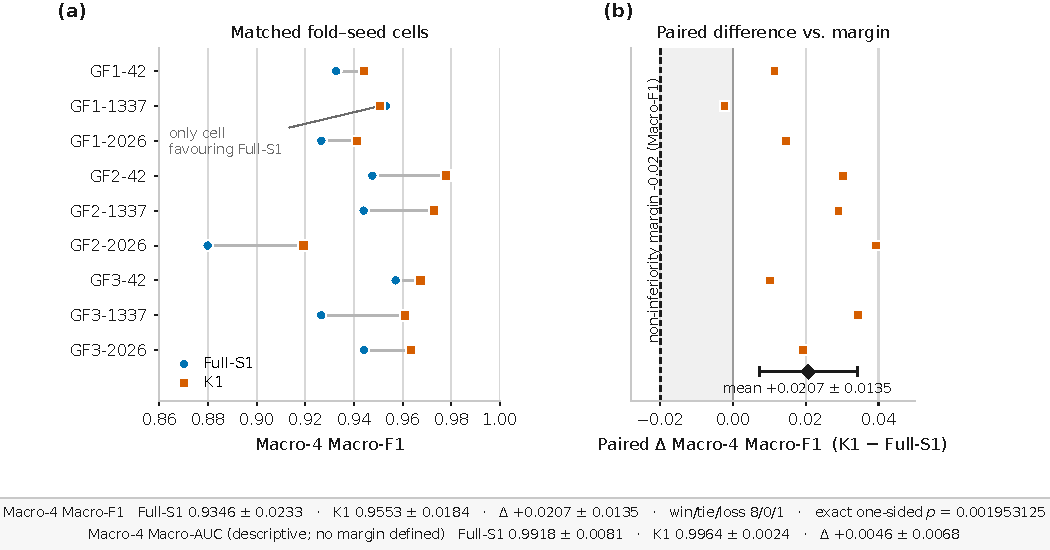
\includegraphics[width=\textwidth]{figures/fig02_matched_cells.pdf}
  \caption{Matched fold--seed comparison of Full-S1 and K1 on the sealed TEST
  partition. (a) Macro-4 Macro-F1 in each of the nine matched cells, with the
  connecting segment showing the paired change. (b) The nine paired differences
  relative to the prespecified $-0.02$ Macro-F1 non-inferiority margin (dashed);
  the diamond marks the mean $\pm$ sample SD of the paired difference. The
  margin was defined for Macro-F1 only: the Macro-AUC values quoted below the
  panels are descriptive, and no non-inferiority margin was specified for them.}
  \label{fig:matched_cells}
\end{figure}


Table~\ref{tab:main_results} summarizes the primary sealed TEST result. Full-S1 obtains a Macro-4 Macro-F1 of $0.934644\pm0.023258$, whereas K1 obtains $0.955334\pm0.018393$. The mean paired change is therefore $+0.020691\pm0.013509$. Eight of the nine matched fold--seed cells favour K1 and one favours Full-S1. Macro-4 Macro-AUC follows the same overall direction, increasing from $0.991793\pm0.008102$ to $0.996398\pm0.002367$ with a paired mean change of $+0.004606\pm0.006794$.

The cell-level values in Table~\ref{tab:matched_cells}, plotted in Figure~\ref{fig:matched_cells}, are important because the aggregate mean does not arise from one isolated run. Positive K1 Macro-F1 differences occur in all three folds, and the largest gain appears in fold 2 / seed 2026 ($+0.039324$). The only negative Macro-F1 cell is fold 1 / seed 1337 ($-0.002303$), a magnitude far inside the predefined acceptable-loss margin. This paired pattern supports the interpretation that K1's performance retention is reproducible across the registered fold--seed design rather than being attributable to a single selected checkpoint.

The observed mean is higher for K1, but the study was designed as a non-inferiority experiment rather than a universal superiority claim. The result therefore supports the narrower conclusion that substantial structural reduction was achieved without an unacceptable aggregate performance loss. The positive point estimate and the gated superiority test are useful additional evidence, but they do not imply that K1 must outperform Full-S1 for every dataset, fold, seed, or future operating condition.

\subsection{Dataset-Level Performance}
\label{subsec:dataset_results}

\begin{table}[t]
\centering
\caption{Dataset-level Macro-F1 for Full-S1 and K1. Values are mean $\pm$ sample SD across the nine matched cells.}
\label{tab:dataset_results}
\small
\begin{tabular}{lccc}
\toprule
Dataset & Full-S1 & K1 & Paired $\Delta$ \\
\midrule
CWRU & $0.854747 \pm 0.083579$ & $0.918945 \pm 0.073432$ & $+0.064198 \pm 0.044152$ \\
JNU & $0.971429 \pm 0.042857$ & $0.980952 \pm 0.037796$ & $+0.009524 \pm 0.028571$ \\
HIT & $0.991039 \pm 0.017798$ & $0.988728 \pm 0.016133$ & $-0.002311 \pm 0.007427$ \\
MaFaulDa & $0.921360 \pm 0.016432$ & $0.932712 \pm 0.017321$ & $+0.011352 \pm 0.019450$ \\
\bottomrule
\end{tabular}
\end{table}

\begin{table}[t]
\centering
\caption{Dataset-level Macro-AUC for Full-S1 and K1. Values are mean $\pm$ sample SD across the nine matched cells. Dataset-level values are descriptive rather than separate confirmatory tests.}
\label{tab:dataset_results_auc}
\small
\begin{tabular}{lccc}
\toprule
Dataset & Full-S1 & K1 & Paired $\Delta$ \\
\midrule
CWRU & $0.974093 \pm 0.033643$ & $0.990379 \pm 0.009921$ & $+0.016286 \pm 0.027983$ \\
JNU & $0.999559 \pm 0.001323$ & $1.000000 \pm 0.000000$ & $+0.000441 \pm 0.001323$ \\
HIT & $0.999969 \pm 0.000094$ & $0.999602 \pm 0.001082$ & $-0.000366 \pm 0.001095$ \\
MaFaulDa & $0.993549 \pm 0.006247$ & $0.995611 \pm 0.004732$ & $+0.002062 \pm 0.003131$ \\
\bottomrule
\end{tabular}
\end{table}

% Figure 3 — dataset-level performance.
% Asset generated by scripts/publication_figures/fig03_dataset_level.py
\begin{figure}[tb]
  \centering
  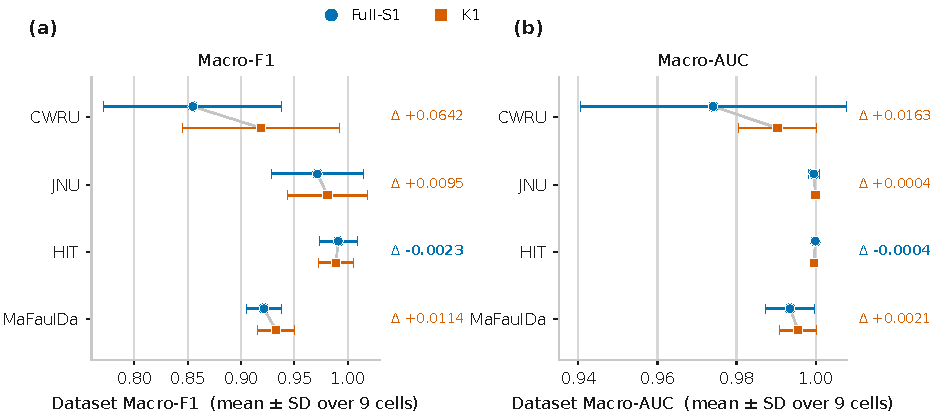
\includegraphics[width=\textwidth]{figures/fig03_dataset_level.pdf}
  \caption{Dataset-level performance of Full-S1 and K1: (a) Macro-F1 and
  (b) Macro-AUC, each shown as the mean over the nine matched fold--seed cells
  with sample-SD whiskers. $\Delta$ is the paired mean difference
  (K1 $-$ Full-S1). HIT is the only dataset whose mean decreases under K1, on
  both endpoints. Dots rather than bars are used because both axes are
  truncated and do not begin at zero.}
  \label{fig:dataset_level}
\end{figure}


Figure~\ref{fig:dataset_level} shows both endpoints per dataset. The largest dataset-level change occurs on CWRU, where mean Macro-F1 increases from $0.854747$ to $0.918945$, a paired improvement of $+0.064198$. CWRU is also the dataset with the largest between-cell variability for both models. This is consistent with the observation that its fault categories remain more sensitive to the chosen split and seed than the near-saturated JNU and HIT tasks. The corresponding CWRU Macro-AUC increases by $+0.016286$.

JNU shows a smaller positive mean change in Macro-F1 ($+0.009524$). Eight of the nine JNU cells are ties at the reported precision and one favours K1, while the mean Macro-AUC changes from $0.999559$ to $1.000000$. This near-ceiling behaviour limits the amount of improvement that can be expressed numerically. MaFaulDa also improves on average, with Macro-F1 increasing by $+0.011352$ and Macro-AUC by $+0.002062$. Because MaFaulDa contains ten classes and a wider variety of machine conditions, preserving or improving its performance after structural reduction is particularly relevant to the claim that one compact encoder can continue to serve heterogeneous label spaces.

HIT is the exception to the otherwise positive dataset means. Its Macro-F1 decreases slightly from $0.991039$ to $0.988728$ ($-0.002311$), and Macro-AUC decreases by $-0.000366$. The absolute level remains high, but this negative delta is important because it prevents the aggregate result from being interpreted as universal dominance. K1's benefit is therefore best described as retained aggregate performance with favourable mean behaviour on three datasets, rather than guaranteed improvement on every constituent domain.

The class-level reports stored with the frozen evaluation further show that the weaker CWRU behaviour is concentrated in confusions among bearing-fault categories rather than a collapse of the entire representation; Section~\ref{subsec:confusion_analysis} examines this structure directly. These class-level differences motivate future work on stronger inter-class separation, but they do not change the main compression result: K1 retains the multi-dataset diagnostic role while using substantially fewer temporal-direction parameters.

\subsection{Aggregated Confusion-Matrix Analysis}
\label{subsec:confusion_analysis}

% -----------------------------------------------------------------------------
% Aggregated confusion-matrix figure (Full-S1 vs K1).
%
% Asset: figures/fig_confusion_aggregated_fulls1_vs_k1.pdf
%   natural size 7.16in x 8.71in, vector, generated by
%   scripts/generate_confusion_figure.py in the publication repository.
%   Provenance and verification:
%   figures/confusion_matrices/confusion_matrix_aggregation_manifest.md
%
% A plain `figure' float is used: the manuscript is single-column, so figure*
% gains nothing here and a separate float class would not be guaranteed to keep
% its numbering position relative to the other figures. Switch to figure* if the
% manuscript is migrated to a two-column journal class.
% keepaspectratio with a height cap leaves room for the caption and lets the
% float shrink for classes with a shorter text block; it does not bind here.
% -----------------------------------------------------------------------------
\begin{figure}[p]
  \centering
  \includegraphics[width=\textwidth,height=0.78\textheight,keepaspectratio]%
    {figures/fig_confusion_aggregated_fulls1_vs_k1.pdf}
  \caption{Aggregated class-level confusion matrices for Full-S1 (left column)
  and K1 (right column) on the four evaluation datasets: CWRU, JNU, HIT and
  MaFaulDa. For each dataset and model, the raw confusion counts of the nine
  matched fold--seed evaluation cells were summed element-wise, and the pooled
  matrix was then normalized by true class; each row therefore shows the
  distribution of predictions conditional on the true class, and all panels
  share the same $0$--$100\%$ colour scale; exactly-zero cells are left blank.
  The pooled matrices are descriptive summaries of the nine matched model
  evaluations rather than a single independent test split; all inferential
  comparisons rest on the paired fold--seed analysis reported in
  Section~\ref{subsec:ni_results}.}
  \label{fig:confusion_aggregated}
\end{figure}


The dataset-level scores above establish that K1 retains the predictive
behaviour of Full-S1, but they do not localize where the two models differ.
Figure~\ref{fig:confusion_aggregated} provides that view. For each dataset and
model, the raw confusion counts of the nine matched fold--seed cells were summed
element-wise and the pooled matrix was then normalized by true class, so that
each row shows the distribution of predictions conditional on the true class.
These matrices are descriptive summaries of the nine matched evaluations rather
than an additional inferential test; the retention claim continues to rest on
the paired analysis reported in Section~\ref{subsec:ni_results}.

The clearest difference appears on CWRU, the dataset with the largest paired
Macro-F1 improvement. Recall of the \texttt{inner\_race} class rises from
approximately $77.3\%$ to $84.6\%$, while the dominant off-diagonal term,
\texttt{inner\_race} predicted as \texttt{outer\_race}, falls from roughly
$20.6\%$ to $15.2\%$. This reduction in inner-/outer-race confusion is
consistent with, and likely contributes to, the improved CWRU Macro-F1 of K1.
It also makes the preceding qualitative statement concrete: the weaker CWRU
behaviour of Full-S1 is concentrated in one specific race-fault confusion rather
than distributed across the three-class CWRU label space.

JNU and HIT are near-diagonal for both models, consistent with their near-ceiling
dataset-level scores. For JNU the pooled sample count is small ($n=216$ across
all nine cells), so a single window shifts a row entry by several percentage
points and the small differences visible between the two columns should not be
over-interpreted. HIT is informative for the opposite reason: it is the one
dataset whose mean Macro-F1 decreases under K1, and the pooled matrices localize
that decrease to class~1, the inner-ring fault condition, whose recall moves
from about $97.3\%$ to $96.6\%$. The class-level evidence therefore supports the
non-inferiority reading developed in Section~\ref{subsec:ni_results}, in which
compression leaves already-strong behaviour essentially intact, rather than a
claim that K1 improves on every dataset and every class.

MaFaulDa remains the most fine-grained task, and its panels show that the
residual errors stay localized to a small number of physically adjacent class
pairs rather than spreading across the ten-class label space. The most
persistent of these is the confusion between \texttt{overhang/cage\_fault} and
\texttt{overhang/outer\_race}, which is almost unchanged between the two models:
$11.5\%$ of true \texttt{overhang/cage\_fault} windows are assigned to
\texttt{overhang/outer\_race} under both Full-S1 and K1, and the reverse
confusion moves only from $19.4\%$ to $17.4\%$. That this pattern survives
compression largely intact suggests that it is intrinsic to the dataset rather
than induced by the reduced model. Taken together, the class-level analysis
supports the view that the performance retention of K1 is not an artefact of
scalar summaries: the lightweight model preserves the qualitative error
structure of the Full-S1 baseline and, on CWRU in particular, reduces one of its
most persistent confusion patterns.

\subsection{Performance Retention and Non-Inferiority}
\label{subsec:ni_results}

The predefined primary margin was $-0.02$ Macro-F1. The observed mean paired difference, $+0.020691$, is therefore $0.040691$ above the non-inferiority boundary after margin shifting. Exact enumeration of all 512 sign patterns gives a one-sided non-inferiority $p$-value of $0.001953125$, the minimum attainable value with nine matched cells under this procedure. The non-inferiority criterion is consequently satisfied.

Because the non-inferiority gate passed, the frozen analysis also reports a two-sided exact sign-flip test for superiority, yielding $p=0.0078125$. This secondary result is supportive, but it should be interpreted in the context of the small number of paired units and the study's original objective. No confidence interval for the paired difference was pre-registered, and none is introduced post hoc as a confirmatory quantity. The strongest statistically aligned statement is therefore that K1 is non-inferior to Full-S1 at the predefined $-0.02$ Macro-F1 margin.

The paired design is important for this conclusion. Rather than comparing two independently averaged collections of runs, each K1 outcome is linked to a Full-S1 outcome from the same global fold and seed. The resulting $\Delta_{f,s}$ values partially control fold and stochastic-training variability and make the sign-flip test operate on the same experimental units that generated the models. This is a more direct measure of compression retention than comparing two unpaired grand means.

\subsection{Computational Efficiency}
\label{subsec:efficiency_results}

\begin{table}[t]
\centering
\caption{Authoritative publication efficiency comparison. Latency/throughput values use the corrected inference-mode benchmark.}
\label{tab:efficiency}
\small
\begin{tabular}{lrrr}
\toprule
Metric & Full-S1 & K1 & Reduction / speed-up \\
\midrule
Encoder parameters & 2,382,033 & 1,375,953 & 42.24\% \\
FP32 state-dict size & 9.135 MiB & 5.286 MiB & 42.14\% \\
Macro-4 computation & 2.6067 GFLOP & 1.4236 GFLOP & 45.38\% \\
CPU b1 model-only & 54.709 ms & 28.560 ms & 1.916$\times$ \\
CPU b1 end-to-end & 55.699 ms & 29.725 ms & 1.874$\times$ \\
GPU b1 model-only & 7.711 ms & 4.164 ms & 1.852$\times$ \\
GPU b1 end-to-end & 9.577 ms & 5.864 ms & 1.633$\times$ \\
GPU b32 throughput & 392.85 win/s & 785.47 win/s & 1.999$\times$ \\
CPU b32 throughput & 13.84 win/s & 26.27 win/s & 1.897$\times$ \\
GPU peak memory & 29.466 MiB & 24.823 MiB & 15.76\% \\
\bottomrule
\end{tabular}
\end{table}

% Figure 5 — computational efficiency.
% Asset generated by scripts/publication_figures/fig05_efficiency.py
\begin{figure}[!tb]
  \centering
  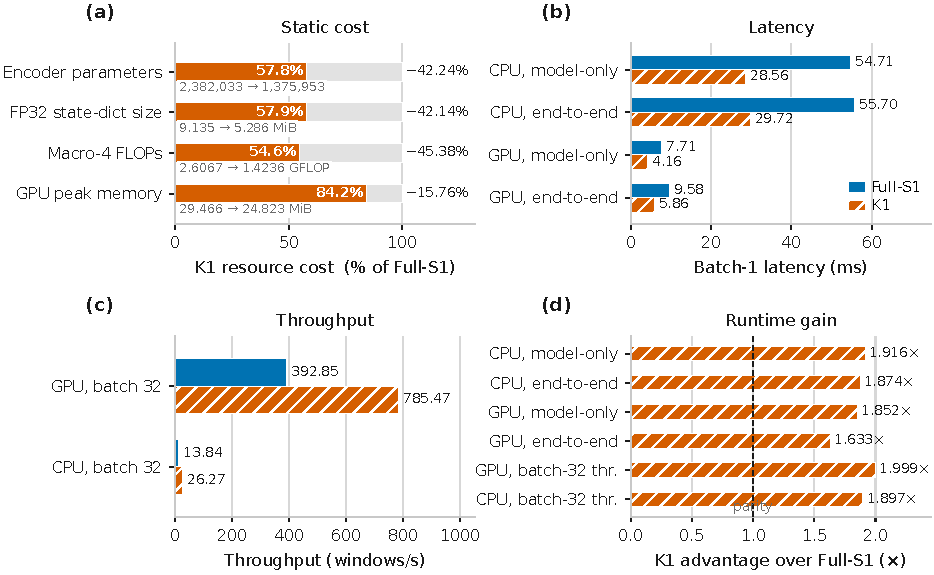
\includegraphics[width=\textwidth]{figures/fig05_efficiency.pdf}
  \caption{Computational efficiency of K1 relative to Full-S1.
  (a) Static resource cost as a percentage of Full-S1, with the absolute values
  beneath each bar. (b) Batch-1 latency for both devices and both measurement
  scopes. (c) Batch-32 throughput. (d) The K1 advantage expressed as a ratio,
  against a parity line at $1.0$. All latency and throughput values come from
  the corrected inference-mode benchmark measured on one deterministically
  selected fold--seed pair; because the selective scan is the reference
  pure-PyTorch recurrence rather than a fused kernel, absolute times are
  specific to this software stack.}
  \label{fig:efficiency}
\end{figure}


Figure~\ref{fig:efficiency} summarises the comparison. The structural change produces substantial reductions before any quantization is applied. K1 contains 1,375,953 encoder parameters compared with 2,382,033 for Full-S1, a $42.24\%$ reduction. Complete-model FP32 state-dictionary size falls by $42.14\%$, from 9.135 to 5.286~MiB. Equal-domain compute decreases by $45.38\%$, from 2.6067 to 1.4236~GFLOP per one-second window. These reductions are consistent with the design: removing one of two independently parameterized state-space directions eliminates a large part of the temporal backbone while leaving the shared stem, coordinate encoder, mixer, and heads intact.

The corrected latency benchmark shows that this reduction translates into real runtime improvements on both CPU and GPU. CPU batch-1 model-only latency decreases from 54.709 to 28.560~ms ($1.916\times$), while end-to-end latency decreases from 55.699 to 29.725~ms ($1.874\times$). GPU model-only latency falls from 7.711 to 4.164~ms ($1.852\times$), and end-to-end latency from 9.577 to 5.864~ms ($1.633\times$). At batch 32, GPU throughput is effectively doubled, from 392.85 to 785.47 windows/s, and CPU throughput increases from 13.84 to 26.27 windows/s.

GPU peak allocated memory decreases by $15.76\%$, which is smaller than the parameter-size reduction because activations and runtime buffers remain present for both models. The difference between parameter reduction and memory reduction illustrates why deployment evidence should not rely on parameter count alone.

An audit after the original efficiency run identified that the first latency/throughput timing path had omitted \texttt{torch.inference\_mode()} despite the benchmark plan stating that it should be active. The frozen historical run was preserved for provenance and a separate correction benchmark was executed on the same representative checkpoint pair and validation inputs. The corrected values in Table~\ref{tab:efficiency} are therefore the authoritative publication numbers. The correction reduced absolute latency for both models and revised the CPU speed-up from roughly $2.2\times$ to roughly $1.9\times$, while leaving the qualitative conclusion unchanged. This correction is reported because inference benchmarking is sensitive to execution context, and preserving the audit trail is preferable to silently replacing the original measurement.

The timing results should also be interpreted relative to the implementation. The selective scan is the reference pure-PyTorch recurrence rather than a fused Mamba kernel. The reported ratios are valid for the common stack used in this study, but absolute milliseconds and potentially some relative speed-ups may change under optimized kernels or different hardware. The results therefore demonstrate deployment-oriented efficiency rather than a universal hardware speed claim.

\subsection{Secondary Q8 Deployment Extension}
\label{subsec:q8_results}

\begin{table}[t]
\centering
\caption{Secondary Q8 deployment extension. The predictive non-inferiority result applies to the weight-only simulated Q8 representation, not to the CPU-dynamic deployment artifact.}
\label{tab:q8}
\small
\begin{tabular}{lrrr}
\toprule
Metric & K1 FP32 & Q8(K1) & Change \\
\midrule
Macro-4 Macro-F1 & $0.955334 \pm 0.018393$ & $0.955334 \pm 0.018405$ & $-0.0000009 \pm 0.0001101$ \\
Macro-4 Macro-AUC & $0.996398 \pm 0.002367$ & $0.996395 \pm 0.002376$ & $-0.0000031 \pm 0.0000156$ \\
Stored model size & 5.285 MiB & 1.526 MiB & $-71.12\%$ \\
CPU b1 model-only latency & 31.046 ms & 28.647 ms & 1.084$\times$ \\
CPU b32 throughput & 26.56 win/s & 27.34 win/s & 1.029$\times$ \\
Parameters & 1,379,813 & 1,379,813 & unchanged \\
\bottomrule
\end{tabular}
\end{table}

% Figure 6 — secondary Q8(K1) extension.
% Asset generated by scripts/publication_figures/fig06_q8.py
\begin{figure}[tb]
  \centering
  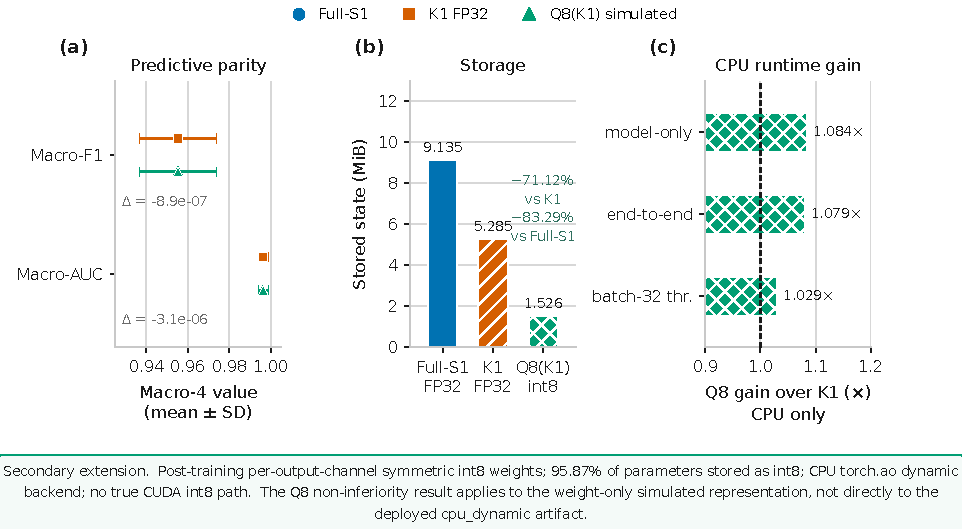
\includegraphics[width=\textwidth]{figures/fig06_q8_extension.pdf}
  \caption{Secondary Q8(K1) deployment extension. (a) The weight-only simulated
  Q8 representation matches K1 FP32 on both Macro-4 endpoints, with paired mean
  differences of order $10^{-6}$ or smaller. (b) Stored state-dictionary size
  for the representative fold--seed cell. (c) CPU runtime gain of Q8 over K1,
  measured within the Q8 benchmark, against a parity line. The predictive
  result applies to the simulated weight-only representation and does not
  transfer automatically to the deployed \texttt{cpu\_dynamic} artifact; no GPU
  int8 execution path exists on the preserved stack.}
  \label{fig:q8}
\end{figure}


Figure~\ref{fig:q8} separates the three aspects of the extension. The Q8 stage changes storage precision without changing the model architecture or parameter count. On the registered \texttt{sim} accuracy representation, Macro-4 Macro-F1 changes from $0.955334\pm0.018393$ for K1 FP32 to $0.955334\pm0.018405$ for Q8, with a mean paired difference of only $-9\times10^{-7}$. Six of nine cells are exactly tied at the reported Macro-F1 precision. The historically defined $-0.01$ non-inferiority criterion is satisfied by the same exact one-sided sign-flip procedure ($p=0.001953125$).

The principal Q8 benefit is storage. The standardized K1 state decreases from 5.285~MiB to 1.526~MiB, a $71.12\%$ reduction or $3.46\times$ compression relative to K1. Relative to Full-S1, the Q8 state is $83.29\%$ smaller, corresponding to approximately $5.99\times$ lower stored size. In contrast, runtime improvement on the real CPU dynamic-quantization backend is modest: model-only batch-1 latency improves from 31.046 to 28.647~ms ($1.084\times$), and batch-32 throughput from 26.56 to 27.34 windows/s ($1.029\times$). This difference between storage and runtime is expected because the selective-scan recurrence and several sensitive modules remain FP32.

Two boundaries are essential when interpreting Q8. First, the preserved implementation does not offer a true INT8 CUDA path. Timing the simulated representation on the GPU would therefore measure FP32 arithmetic on dequantized weights and would not constitute an INT8 acceleration result; no such claim is made. Second, the TEST accuracy evaluation applies to \texttt{sim}, whereas the CPU deployment model uses dynamic activation quantization in addition to int8 weights. On validation data, these two representations agree on 98.63\% of top-1 predictions in the equal-domain summary, but agreement falls to 95.0\% on MaFaulDa, where the maximum absolute probability difference reaches 0.49. Consequently, the formal Q8 non-inferiority result does not automatically transfer to the deployed \texttt{cpu\_dynamic} artifact. A future pre-registered evaluation of the exact deployed representation would be required to make that stronger claim.

Taken together, the three-stage result distinguishes two mechanisms. Structural compression from Full-S1 to K1 delivers most of the compute and latency reduction, whereas post-training Q8 contributes mainly a further storage reduction. This separation is useful for deployment decisions because it avoids treating weight precision and architecture size as interchangeable sources of efficiency.

\subsection{Comparison with Related Approaches}
\label{subsec:comparison}

\begin{table}[t]
\centering
\caption{Qualitative positioning against representative related work. A check mark indicates that the cited work explicitly addresses the corresponding dimension; the table is not an accuracy leaderboard.}
\label{tab:related_work}
\scriptsize
\resizebox{\textwidth}{!}{%
\begin{tabular}{lcccccccl}
\toprule
Work & Reusable / multi-dataset & Mamba/SSM & Structural compression & KD & Multi-teacher & Quantization & Physical edge & Main distinction \\
\midrule
FaultFormer \citep{Zhou2024FaultFormer} & \checkmark & -- & -- & -- & -- & -- & -- & SSL/adaptation, not deployment compression \\
BearingFM \citep{Lai2024BearingFM} & \checkmark & -- & -- & -- & -- & -- & concept & Foundation-style bearing representation \\
RmGPT \citep{Wang2025RmGPT} & \checkmark & -- & -- & -- & -- & -- & -- & Unified diagnosis/prognosis model \\
VibFM \citep{Mannone2026VibFM} & \checkmark & -- & -- & -- & -- & -- & -- & 16-dataset masked spectrogram pretraining \\
MD-BiMamba \citep{Wang2025MDBiMamba} & -- & \checkmark & -- & -- & -- & -- & -- & Bidirectional Mamba diagnosis \\
VibrMamba \citep{Yi2025VibrMamba} & multi-task & \checkmark & lightweight design & -- & -- & -- & -- & Lightweight Mamba designed directly \\
DTCP-MAKD \citep{Zhong2024DTCPMAKD} & -- & -- & \checkmark & \checkmark & assistants & -- & -- & Channel pruning + teacher assistants \\
BFD-KD \citep{Sun2026BFDKD} & -- & -- & lightweight student & \checkmark & \checkmark & -- & -- & Multi-teacher rolling-bearing KD \\
BearingPGA-Net \citep{Liao2024BearingPGANet} & -- & -- & compact student & \checkmark & -- & \checkmark & \checkmark & KD + quantization + FPGA \\
\textbf{PC-STE/K1 (this work)} & \checkmark & \checkmark & \checkmark & \checkmark & seed ensemble & Q8 secondary & -- & Shared encoder + direction reduction + paired retention test \\
\bottomrule
\end{tabular}%
}
\end{table}


Table~\ref{tab:related_work} is intended as a positioning comparison rather than a numerical leaderboard. Direct accuracy, latency, and FLOP comparisons across these papers would be misleading because datasets, split protocols, input lengths, hardware, and software kernels differ substantially. Instead, the table identifies which research dimensions each work explicitly addresses.

The closest architecture-centric comparison is VibrMamba, which establishes lightweight bidirectional Mamba-based rotating-machinery diagnosis across several classification tasks \citep{Yi2025VibrMamba}. The distinction is that K1 is obtained by compressing an already trained shared encoder and is evaluated against its own matched Full-S1 reference. MD-BiMamba establishes bidirectional Mamba processing in bearing diagnosis but does not study the same teacher-to-forward-student compression problem \citep{Wang2025MDBiMamba}. On the compression side, DTCP-MAKD and BFD-KD demonstrate structural or multi-teacher distillation strategies, but their teacher construction and model roles differ from the same-architecture seed ensemble used here \citep{Zhong2024DTCPMAKD,Sun2026BFDKD}. BearingPGA-Net provides stronger evidence of physical embedded deployment through FPGA acceleration and therefore bounds the present claim to \emph{deployment-oriented} benchmarking rather than physical edge deployment \citep{Liao2024BearingPGANet}.

Foundation-style approaches such as FaultFormer, BearingFM, RmGPT, and VibFM show that reusable or pretrained vibration representations are already established \citep{Zhou2024FaultFormer,Lai2024BearingFM,Wang2025RmGPT,Mannone2026VibFM}. PC-STE/K1 is not positioned as a larger or more general foundation model than these approaches. Its contribution is narrower: it studies how a shared multi-dataset state-space representation can be structurally compressed, distilled, and evaluated as a paired performance-retention problem with explicit computational measurement.

\subsection{Discussion and Limitations}
\label{subsec:limitations}

The result that K1's mean Macro-F1 is higher than Full-S1 may initially appear counterintuitive because K1 removes half of the directional temporal paths. One plausible explanation is that the structural reduction acts as a form of regularization while the three-teacher ensemble provides a smoother target distribution than any single teacher. Removing the reverse path may also reduce optimization burden on these relatively short patch sequences. However, the experiment was not designed to isolate these mechanisms, and the observed improvement should not be presented as proof of causality. The defensible conclusion is empirical: the removed direction was not necessary to retain aggregate performance under the registered protocol.

Several limitations bound the scope of the result. First, the four datasets provide heterogeneous benchmark conditions but do not constitute an unseen-machine evaluation. In CWRU, the final split is cross-load on the same rig; JNU and HIT similarly do not establish transfer to an entirely new machine and sensing system. The work therefore evaluates a shared multi-dataset model under frozen within-dataset protocols, not universal machinery generalization.

Second, the computational benchmark uses one deterministically selected fold--seed model pair on one workstation-class CPU/GPU system. This controls model choice and permits reproducible within-host comparisons, but it does not capture variation across embedded processors, other GPUs, or optimized inference runtimes. The pure-PyTorch selective scan is particularly relevant: a fused Mamba implementation could change absolute latency and may change the relative benefit of removing a direction.

Third, Q8 is a secondary extension with a deliberate separation between the predictive and deployed representations. The registered \texttt{sim} representation supports the non-inferiority result, whereas the actual CPU dynamic-quantization artifact has only validation-level agreement measurements. No Q8 GPU acceleration is available on the preserved stack. These constraints mean that Q8 currently supports a strong storage-compression statement and a modest CPU deployment observation, but not a fully validated INT8 edge-deployment claim.

Finally, the aggregate metric hides differences in dataset difficulty. CWRU remains substantially more variable than JNU and HIT, and some bearing-fault classes remain harder to separate. Future work should therefore investigate representations and objectives that improve class separation without sacrificing the shared-encoder design, and should extend evaluation to genuinely unseen machines or acquisition systems.
